\documentclass[12pt, a4paper, final]{report}
\usepackage[nottoc,section]{tocbibind}
\usepackage[titles]{tocloft}
\usepackage{palatino}
\usepackage{parskip}
\usepackage{amsmath}
\usepackage{alltt}
\usepackage{booktabs}
\usepackage{algorithmicx}
\usepackage{algpseudocode}
\usepackage{algorithm}
\usepackage{mathabx}
\usepackage{graphicx}
\usepackage{epstopdf}
\usepackage{multirow}
\usepackage{minted}
\usepackage{dsfont}
\usepackage{color}
\usepackage{url}

\begin{document}

% -- Title --
\title{An Exploration of Modern Cryptography}
\author{Siddharth Mahendraker\\
        \texttt{siddharth\_mahen@me.com}}
\date{2012}
\maketitle

% -- Abstract --
\begin{abstract}
In this paper we analyze three cryptographic algorithms spanning
all three major branches of modern cryptography: substitution ciphers,
block ciphers and public-key ciphers. We explore cryptanalytic techniques used
to break each algorithm, and evaluate each algorithm with regard to its
practicality, speed and memory efficiency.
\end{abstract}

% -- Bookkeeping
\setcounter{secnumdepth}{3}
\renewcommand{\thesection}{\arabic{section}}
\renewcommand{\cftsecfont}{\bfseries}
\settocbibname{References}
\setlength\cftbeforesecskip{3pt}
\setlength\cftbeforesubsecskip{3pt}

% -- Easier text in matricies
\newcommand{\ptm}[2]{\Pr\begin{pmatrix}
\text{\scriptsize#1}\\
\text{\scriptsize#2}
\end{pmatrix}}

% -- Easier footnotes
\newcounter{fn}
\newcommand{\fnt}[1]{%
\addtocounter{fn}{1}%
\footnote[\value{fn}]{#1}}

% -- ToC --
\setcounter{page}{1}
\pagenumbering{roman}
\tableofcontents
\clearpage
\addcontentsline{toc}{section}{Introduction}
\setcounter{page}{1}
\pagenumbering{arabic}

% -- Intro --
\section*{Introduction}

Suppose two people, Alice and Bob, wish to communicate by mail and do not
want their mail woman, Eve, to be able to read their messages. Alice and Bob
are military personal of the same country, but they have never met each
other before. Because Eve is the mail woman, she will be able to read
all of the messages passing between Alice and Bob, but her obligation to
the postal service prevents her from tampering with these
messages\fnt{In reality, Eve would not be bound by such a petty
obligation, however, for the sake of simplicity, let us assume this is
true.}.

The question is, is it possible for Alice and Bob to communicate securely
in these circumstances? Astoundingly, the answer is yes!

Cryptography is the science of securely sending messages over insecure
channels. Using cryptographic techniques, Alice and Bob can be sure that
their communications are illegible to Eve.

\subsection{Terminology and Basic Concepts}

\subsubsection{Alice and Bob}
Unless specified otherwise, Alice and Bob are two parties attempting to
communicate over an insecure channel, and Eve is their adversary trying to
read their messages.

\subsubsection{Encryption and Decryption}

Messages in cryptography are formally called plaintext. When messages are
scrambled, or made ``illegible'', they are encrypted. The encrypted form
of these messages is called ciphertext. The reverse process of encryption,
decryption, accepts ciphertext as input and returns plaintext. We can
describe this mathematically as:
\begin{align*}
    E(M) & = C\\
    E'(C) & = D(C) = M
\end{align*}
Where $M$ denotes plaintext, $C$ denotes cipher text, $E$ is the encryption
function and $D$ is the decryption function, or the inverse of $E$. Also
note the following identity:
\begin{align*}
    D(E(M)) & = M\\
    E(D(C)) & = C
\end{align*}

\subsubsection{Ciphers and Keys}

A cryptographic algorithm, or cipher, is a function used for encryption
and decryption.

If the workings of a cipher are made public, then the messages
of anyone who is known to use the cipher can quickly be compromised
by simply implementing an inverse of the cipher. Therefore, cryptographers
introduced a key. A key is a piece of secret, private information
upon which the cipher depends. It often takes the form of a number.
The total number of possible values a key can take on is called the
keyspace. Because ciphers depend on the key to encrypt and decrypt
plaintext, encryption and decryption is often denoted:
\begin{align*}
    E_K(P) & = C\\
    D_K(C) & = P
\end{align*}
The key is denoted by $K$ and the keyspace is by $\mathcal{K}$. Note that
the identity mentioned in 0.1.2 still holds true for ciphers.

\subsubsection{Symmetric and Public-Key Ciphers}

There are two distinct kinds of ciphers, symmetric ciphers and public-key
(or asymmetric) ciphers.

Symmetric ciphers are ciphers for which the key used to decrypt ciphertext
and encrypt plaintext is the same. In most symmetric ciphers, this means
that Alice and Bob will need to agree on a key before they can begin
sending messages. Symmetric ciphers can be further categorized as stream
ciphers or block ciphers. Stream ciphers operate on only one bit (or byte)
of plaintext at a time, where as block ciphers operate on a large number
of bytes at once.

Public-key ciphers are ciphers for which the key used for encrypting
plaintext is different from the key used for decrypting ciphertext.
Further, these keys should be independent of each other, meaning the
decryption key can not be calculated\fnt{In a feasible amount of time,
i.e.\ less than the age of the universe.} from the encryption key.
The design of this cipher is such that the encryption key can be published
for anyone to encrypt messages with, but only the owner of the decryption key
can decrypt these message. This is why the encryption key is referred to as the
public key and the decryption key is referred to as the private key.

\subsubsection{Cryptanalysis}

Cryptanalysis is the study of obtaining the plaintext from encrypted
messages without the knowledge of the key. An attempt to cryptanalyze
a cipher is called an attack. Successful attacks reveal either the
plaintext, the secret key, or both.

The only assumption made in cryptanalysis is that the only piece of
information the users of the cipher, Alice and Bob know that the adversary
Eve does not is the secret key. This means that all other information,
including communications and the workings of their cryptographic algorithm
are available to anyone. This assumption implies that the security of
the algorithm rests only in the key, and nothing else.

There are three main cryptanalysis techniques we will be focusing on in
this report. Listed in decreasing order of difficulty they are; ciphertext
only attacks, known-plaintext attacks and chosen plaintext attacks.

In ciphertext only attacks, the cryptanalyst (or attacker) Eve has access
to several different ciphertexts. The attack is considered successful if
Eve successfully retrieves the plaintexts corresponding to the ciphertexts
or the key used in encryption.

In known-plaintext attacks, Eve has access to the ciphertexts as well
as their corresponding plaintexts. The attack is successful if Eve
finds the key (or keys) used to encrypt each plaintext.

In chosen plaintext attacks, Eve can not only access the ciphertexts,
and their corresponding plaintext, but can also choose which plaintexts
are encrypted and which are decrypted. The attack is successful if Eve
retrieves the key (or keys) used to encrypt each plaintext.

Note that in all of the cases above, the adversary, Eve, had to know
some amount of ``information'' about the ciphertext, plaintext or the
relationship between the two. The only other technique which can yield
the key is a brute force attack or exhaustive search attack, in which
Eve checks the ciphertext against all possible keys in the keyspace until
one of the keys reveals the plaintext.

% --Caesar Cipher--
\section{Substitution Ciphers}

A substitution cipher is a cipher in which each character or byte in the
plaintext is substituted with a character or byte\fnt{A byte
is a group of 8 binary digits, or bits, which are operated on as one
unit. For example, this is the byte representing the integer 5:
\texttt{00000101}.} in the cipher text.

The substitution cipher we will be analyzing is called the Caesar cipher.
The Caesar cipher operates on one byte (or character) of the plaintext at
a time. Briefly, the value of the key is added to each byte of the
plaintext. If this sum is a byte which does not corresponds to a
character in the English alphabet, the sum is set modulo 26\fnt{
Recall that $a \equiv b \pmod{c}$ implies $a = b + ck$, where $k \in
\mathds{Z}^+$. Basically this means the remainder of $a$ divided by $c$.}.
Decryption works the opposite way. The value of the key is subtracted from
each byte of the ciphertext. If the sum is not in the English alphabet,
the sum is set modulo 26.

See the appendix for a full code example.

\subsection{Information Theory and Languages}

Before we begin a deconstruction of the Caesar cipher, there are a few
assumptions we make that must be explained.

Firstly, we must clarify the definition of information we used in section
0.1.5. Information can be rigorously defined as the least number of bits
it would take to represent all possible meanings of a message, assuming
all messages are equally likely.

For example, suppose we are trying to determine the amount of information
in a list of possible sexes:

\begin{enumerate}
\item Male
\item Female
\end{enumerate}

Clearly, this data can be represented using one bit, where the 1
represents male and 0 represents female. Therefore, we can say that there
is only one bit of information present in this list.

Now, if we take a look at words used in the English language, we clearly
see that English does not represent this information very succinctly, i.e.\
there is a considerable amount of redundancy per character.

For example, the sentence ``met u tmrw @ 9'' conveys the same information
as the sentence ``meet you tomorrow at nine'', yet does so much more
succinctly. Therefore, we can say that many of the character in the
latter sentence are redundant or useless.

Although this may not seem related at all to cryptography, it is. This
redundancy in languages causes sentences to ``leak'' more information than
they need to. As we shall soon see, this often manifests itself as
discrepancies in the frequency and location of certain characters in
relation to others, and makes breaking the Caesar cipher a piece of
cake.

\subsection{Cryptanalysis of the Caesar Cipher}

If we take the most naive cryptanalytic approach, a brute force attack,
the Caesar cipher appears quite strong. Indeed the keyspace of the cipher
is $26!$ or approximately $4 \times 10^{26}$. This means that even if we
were to check a million keys per second, it would still take us around
$1.27 \times 10^{13}$ years to check every possible key! That's longer than
the estimated age of the universe!

However, we know from our understanding of redundancy in languages that there
is information being leaked here.

Because the output of this algorithm merely ``switches'' one letter with another,
the letters in any particular ciphertext will continue to follow the known
statistic rules regarding English text. Particularly, they will maintain certain
distributions of characters over the message.

\begin{figure}[h]
\begin{center}
\begin{tabular}{cccc}
\toprule
\multicolumn{4}{c}{Letter Frequency (\%)}\\
\midrule
E & 13.11 & M & 2.55\\
T & 10.47 & U & 2.45\\
A & 8.15  & G & 1.95\\
O & 8.05  & Y & 1.95\\
N & 7.15  & P & 1.96\\
R & 6.85  & W & 1.55\\
I & 6.35  & B & 1.45\\
S & 6.15  & V & 0.95\\
H & 5.25  & K & 0.45\\
D & 3.75  & X & 0.15\\
L & 3.35  & J & 0.15\\
F & 2.95  & Q & 0.15\\
C & 2.75  & Z & 0.05\\
\bottomrule
\end{tabular}
\end{center}
\caption{General frequency of English characters in decreasing order}
\end{figure}

\pagebreak
Therefore, if we are given the following ciphertext:

\begin{alltt}
ofobiyxocryevnkvcyexnobcdkxndrovswsdkdsyxcypmbizdyqbkz
rikckdyyvgroxeconsxmyxtexmdsyxgsdrcyvsnzbyqbkwwsxqzbkm
dsmockxnpsbwwkdrowkdsmkvmyxtomdebocsdmkxlorsqrvioppomd
sforygofobspwscecondrobowkilonsckcdbyecmyxcoaeoxmocsx
mvensxqwkccnkdkdropdybcobfobrsqrtkmusxq
\end{alltt}

We would first construct a table of the characters present in the text and
their respective frequencies, as so:

\begin{figure}[h]
\begin{center}
\begin{tabular}{l*{13}{c}}
\toprule
Character & o & s & c & k & d & x & y & b & m & r & n & e & w\\
\midrule
Frequency & 27 & 21 & 19 & 19 & 19 & 18 & 17 & 15 & 14 & 13 & 10 & 9 & 9\\
\bottomrule
\hfill\\
\toprule
Character & v & q & p & i & f & z & g & t & l & a & u & h & j\\
\midrule
Frequency & 8 & 7 & 6 & 5 & 4 & 4 & 3 & 3 & 2 & 1 & 1 & 0 & 0\\
\bottomrule
\end{tabular}
\end{center}
\caption{Frequency of English characters in the ciphertext}
\end{figure}

Then we would map the most frequent characters to each other, using a
frequency table, found in Figure 1.
Clearly, the character ``o'' appears to represent the character ``e''.
We know, based on our knowledge of the algorithm, that the key was used
as a shift, such that the integer value of each ciphertext character was the
integer value of the plaintext character plus the key. A quick glance at the
ASCII character table reveals that e = 101 and o = 111 as integers.
Therefore, we can conclude that the key used to encrypt this plaintext
is the number 10.

A quick check reveals that we were indeed correct.

\begin{alltt}
everyoneshouldalsounderstandthelimitationsofcryptograp
hyasatoolwhenusedinconjunctionwithsolidprogrammingprac
ticesandfirmmathematicalconjecturesitcanbehighlyeffect
ivehoweverifmisusedtheremaybedisastrousconsequencesin
cludingmassdatatheftorserverhighjacking
\end{alltt}

With proper punctuation and capitalization the plaintext becomes:

\begin{alltt}
Everyone should also understand the limitations of cry
ptography as a tool. When used in conjunction with sol
id programming practices and firm mathematical conject
ures, it can be highly effective. However, if misused,
there may be disastrous consequences, including mass
data theft or server highjacking.
\end{alltt}

\subsection{Advantages and Disadvantages of the Caesar Cipher}

At this point, you may be asking yourself why the Caesar cipher would
ever be considered a viable method of encrypting data, considering we
have been able to break it quite easily using a ciphertext only attack.

Although this cipher is very deeply flawed, it still has certain
advantages which make it practical in certain situations.

For example, if speed and memory are your main concerns, and your
plaintext only has to be superficially secure, then this cipher is one
of your best options. The Caesar cipher has a time complexity of
$\Theta(1)$ and a memory complexity of $\Theta(1)$\fnt{See
\cite[p.~76]{silverman} for a thorough review of Order Notation}.
This means that the cipher's speed and memory usage stay within a constant
range, and do not grow (or shrink) in relation to the size of the cipher's
input. This is because the cipher operates on only one character (or byte)
at a time, and performs the same constant time operation on each byte.

Furthermore, the Caesar cipher may also be practical in situations where
only a small amount of plaintext is being encrypted. The statistical
analysis which was used is only relevant to plaintexts of sufficient
length. It has been shown that highly competent cryptanalysts can break
the Caesar cipher using only 25 English characters of plaintext.
Therefore, the Caesar cipher might be practical for messages shorter than
25 characters.

\section{Block Ciphers}

Block ciphers, unlike substitution ciphers, operate on several bytes at
a time. This ensures that redundancies in the data are not easy
to analyse using statistical methods, such as the frequency analysis
we performed earlier.

The two basic methods of obfuscating redundancies in plaintext
messages are confusion and diffusion. Confusion obscures the relationship
between the plaintext and the ciphertext. This can be most simply achieved
through substitution, as was done in the Caesar cipher. Diffusion, on the
other hand, disperses the redundancy in the plaintext over the ciphertext.
A simple example of this is a permutation box, where the position of the
input bits are swapped with each other.

Substitution ciphers can only use confusion based techniques, whereas block
ciphers are capable of using both confusion and diffusion based techniques.
This is why modern block ciphers are generally more secure than modern
substitution ciphers.

The block cipher we will be analyzing is a heavily modified version of the
GHOST cipher used by the former Soviet Union as encryption standard\fnt{
See \cite[p.~331]{schneier} for information about the original version of this
algorithm.}. The cipher operates on 64 bits of input and accepts a 256 bit key.

See the appendix for a full code example.

\subsection{Construction of Block Ciphers}

Before we begin the analysis of GHOST, let us briefly look at some important
ideas behind the design and construction of block ciphers.

\subsubsection{Feistel Networks}

Most blocks ciphers, including this version of GHOST, are Feistel networks.
In Feistel networks, the plaintext is divided into two separate halves, the
right half, $R$, and the left half, $L$. Encryption is performed by
repeatedly iterating a function, $f$, over half the plaintext, using a
different subkey of $K$ each time, such that the $i$-th left and right half
are defined as:
\begin{align*}
    L_i & = R_{i - 1}\\
    R_i & = L_{i - 1} \oplus f(R_{i - 1}, K_i)
\end{align*}
Decryption is the exact inverse of encryption, except the subkeys for $f$ are
placed in inverse order.
\begin{align*}
    L_i & = R_{i + 1} \oplus f(L_{i + 1}, K_{i + 1})\\
    R_i & = L_{i + 1}
\end{align*}
The wonderful property of this construction, is that decryption does not
require $f$ to be invertible, it can be as complex as desired, so long as
the input to each iteration (or round) can be reconstructed. This means
that rather than having to construct both an encryption and decryption
function, one only needs to construct the former.

For example, consider encrypting the following message, $m = 01011100$, via
a Feistel network, using subkeys $K_1 = 1100, K_2 = 0101$ and the function
$f(x, k) = (x + x) \oplus k$. Breaking $m$ into two halfs, we obtain,
$L_0 = 0101, R_0 = 1100$. Then, passing $L_0$ and $R_0$ into the Feistel
network, we obtain the output byte $01010011$:
\begin{align*}
    L_1 &= 1100\\
    R_1 &= 0101 \oplus f(1100, 1100)\\
        &= 0101 \oplus 0000\\
        &= 0101\\
    L_2 &= 0101\\
    R_2 &= 1100 \oplus f(0101, 0101)\\
        &= 1100 \oplus 1111\\
        &= 0011\\
\end{align*}
Now if we decrypt $01010011$ by passing it in reverse through our
Feistel network, we obtain our orignal message $01011100$.
\begin{align*}
    L_2 &= 0101\\
    R_2 &= 0011\\
    L_1 &= 0011 \oplus f(0101, 0101)\\
        &= 0011 \oplus 1111\\
        &= 1100\\
    R_1 &= 0101\\
    L_0 &= 0101 \oplus f(1100, 1100)\\
        &= 0101 \oplus 0000\\
        &= 0101\\
    R_0 &= 1100
\end{align*}

\subsubsection{S-Boxes and P-Boxes}

The confusion and diffusion properties of block ciphers come from their
substitution boxes and their permutation boxes, abbreviated to S-boxes
and P-boxes respectively. S-boxes output a transformation of their input
bits, while P-boxes output a permutation of their input bits. An S-box
which maps $m$ input bits to $n$ output bits is called an $m \times n$ bit
S-box.

Some ciphers do not have P-boxes, but rather permute the input or output
bits in a different fashion. The GHOST cipher, for example uses an 11-bit
left circular shift, rather than a proper permutation box.

S-boxes are the most important part of any block cipher, because they
provide its only non-linear component. If the S-boxes were linear,
(or close to linear) the entire cipher would just be one big linear
transformation of bits, and hence trivially simple to break.

Therefore, if these boxes are improperly designed, that is, they perform
close to linear transformations of bits, the security of the entire
cipher can be compromised.

As we shall soon see, if these boxes are improperly designed, their overarching
cipher can be susceptible to attack.

\subsection{Linear Cryptanalysis}

Suppose you were given an expression of XOR'd bits, called a linear expression,
of the form:
\begin{align}
    a_1X_1 \oplus a_2X_2 \oplus \cdots \oplus a_nX_n \oplus
    b_1Y_1 \oplus b_2Y_2 \oplus \cdots \oplus b_mY_m = 0
\end{align}
It is obvious that $(1)$ holds true with a probability of $1/2$ if
$\{X\}, \{Y\}, \{a\}$ and $\{b\}$ are all random sequences of bits.

Now suppose that $X$ and $Y$ are the respective sequences of input and
output bits of a substitution box. If the S-box is a good one, then
for any random sequence $\{a\}$ and $\{b\}$, the probability of $(1)$
being $0$ should be less than some $1/2 + \epsilon$, where $\epsilon$ is
some negligibly small number\fnt{In practice a negligible value can be defined
as any value greater than $1/2^{80}$. This ensures that an event that occurs with
this probability probably won't happen over the life of the key.}. However, if
there are certain combinations of $\{a\}$ and $\{b\}$ which result in a
probability of obtaining $0$ significantly greater or significantly less than
$1/2$, then the S-box is said to be biased. The linear probability bias
(or just bias), is the amount from which the probability of the linear
expression deviates from $1/2$. When the bias is positive, the expression is
said to be linear and when it is negative it is said to be affine.

Linear cryptanalysis is a known-plaintext attack against block ciphers,
which attempts to take advantage of highly probable or improbable linear
expressions occurring at key points in the cipher, most importantly in
S-boxes. The attack uses these linear expressions to approximate portions
of the cipher (accurate to some non-negligible probability) and eventually
obtain the key bits. In general, linear cryptanalysis does not reveal the
entire key, but rather makes exhaustive search an option by finding several
key bits.

For example, suppose, given a $4 \times 4$ bit S-box, every combination
of the four input bits are inputed and every output is recorded.
It is found that the XOR of the first and second bits of input and the
fourth bit of the output is equal to $0$ exactly $12$ of $16$ times.
This can be stated as:
\begin{align*}
    X_1 \oplus X_2 \oplus Y_4 & = 0
\end{align*}
Or equivalently:
\begin{align*}
    X_1 \oplus X_2 = Y_4
\end{align*}
With a probability of $3/4$.

Therefore, the probability bias of this expression is $3/4 - 1/2 = 1/4$.
Now suppose that the input to this S-box is the plaintext, $P$, XOR'd with
the key $K$. Then we know that expression $(P_1 \oplus K_1) \oplus (P_2
\oplus K_2) = V_4$ holds true with a probability of $3/4$, where $V$ is the
vector of output bits. Now, if we fix values for the bits $K_1$, $K_2$, and
then XOR these hypothesized values with the output, we obtain our original
plaintext bits.
\begin{align*}
    P_1 \oplus K_1 \oplus P_2 \oplus K_2 \oplus K_1 \oplus K_2 = V_4
    \oplus K_1 \oplus K_2\\
    P_1 \oplus P_2 = V_4 \oplus K_1 \oplus K_2
\end{align*}
If we try each combination of $K_1$ and $K_2$ over several different
pairs of values $P$ and $V$ (called plaintext-ciphertext pairs), we will
see one pair of $K_1$ and $K_2$ which when added give us the plaintext bits
most often, i.e.\ with the probability $3/4$. These values are the values of
the first and second bits of the key. The rest of the key can then be acquired
by exhaustive search of the remaining key bits.

In this example, the savings were quite trivial because the keyspace was only
$2^4$, however, in larger keyspaces, the advantages become more significant.

\subsection{Cryptanalysis of the GHOST Cipher}

Now that we know how linear cryptanalysis works, we can begin analyzing the
GHOST cipher. The GHOST cipher is a 8 round Feistel network which uses a
different S-box for each round. At each iteration of the Feistel network, the
32 bit input XOR'd with the subkey for that round. Then it is split into eight
4 bit chunks, which are each inputed into a different S-box, the first chunk in
the first S-box, and so forth. Finally, these chunks are concatenated and
circularly left shifted 11 bits.

To illustra

During the round, the subkey corresponding
to that round is XOR'd with the input and that is then circularly left shifted
11 bits.

Each S-box is a $4 \times 4$ S-box, meaning it accepts $4$ input bits and $4$
output bits. The first S-box, for example looks like this:
\begin{figure}[h]
\begin{center}
\begin{tabular}{l*{16}{c}}
\toprule
Input (hex) & 0 & 1 & 2 & 3 & 4 & 5 & 6 & 7 & 8 & 9 & A & B & C & D & E & F\\
\midrule
Ouput (hex) & 4 & A & 9 & 2 & D & 8 & 0 & E & 6 & B & 1 & C & 7 & F & 5 & 3\\
\bottomrule
\end{tabular}
\end{center}
\caption{Substitution Box 1}
\end{figure}

To figure out which linear expressions (if any) have high or low biases, we need
to test every combination of input bits and output bits for each S-box, and
find out which match the most or least often. That is, we need to evaluate
\begin{align*}
    a_1X_1 \oplus a_2X_2 \oplus a_3X_3 \oplus a_4X_4 \oplus
    b_1Y_1 \oplus b_2Y_2 \oplus b_3Y_3 \oplus b_4Y_4 = 0
\end{align*}
Or equivalently,
\begin{align*}
    a_1X_1 \oplus a_2X_2 \oplus a_3X_3 \oplus a_4X_4 =
    b_1Y_1 \oplus b_2Y_2 \oplus b_3Y_3 \oplus b_4Y_4
\end{align*}
For every possible combination of $a_i = \{0, 1\}$ and $b_j = \{0, 1\}$.

\begin{figure}[h]
\begin{center}
\begin{tabular}{c|*{16}{c}}
$\oplus$& 0& 1& 2& 3& 4& 5& 6& 7& 8& 9& A& B& C& D& E& F\\
\midrule
0& 8& 0& 0& 0& 0& 0& 0& 0& 0& 0& 0& 0& 0& 0& 0& 0\\
1& 0&-2& 4&-2&-2& 0& 2& 0& 4& 2& 0& 2&-2& 0& 2& 0\\
2& 0& 0&-2& 2&-2& 2& 0& 0&-2& 2& 0& 0&-4&-4& 2&-2\\
3& 0& 2&-2& 0&-4&-2&-2& 0& 2& 0&-4& 2& 2& 0& 0&-2\\
4& 0& 2& 0&-2& 2&-4&-2&-4& 0& 2& 0&-2&-2& 0& 2& 0\\
5& 0& 0& 0& 0& 0&-4& 4& 0& 0& 0& 0& 0& 0&-4&-4& 0\\
6& 0& 2&-2& 0& 0&-2&-2& 4& 2& 0& 4& 2&-2& 0& 0& 2\\
7& 0& 4& 2& 2&-2& 2& 0& 0& 2& 2& 0&-4& 0& 0&-2& 2\\
8& 0& 4& 2&-2& 2& 2& 0& 0&-2& 2& 0& 4& 0& 0&-2&-2\\
9& 0&-2& 2& 4& 0&-2&-2& 0&-2& 4& 0& 2& 2& 0& 0& 2\\
A& 0& 0& 4& 0& 0& 0&-4& 0& 0&-4& 0& 0& 0&-4& 0& 0\\
B& 0&-2& 0&-2&-2& 0&-2& 0& 0& 2& 4&-2& 2& 0&-2&-4\\
C& 0&-2&-2& 0& 0& 2&-2&-4& 2& 0& 0& 2&-2& 0&-4& 2\\
D& 0& 0& 2& 2&-2&-2& 0& 0&-2&-2& 0& 0&-4& 4&-2&-2\\
E& 0& 2& 0& 2&-2& 0& 2&-4& 0&-2& 4& 2& 2& 0& 2& 0\\
F& 0& 0& 0& 4& 4& 0& 0& 0& 4& 0& 0& 0& 0& 0& 0&-4\\
\end{tabular}
\end{center}
\caption{Linear approximation table for S-box 1}
\end{figure}

This can be done using a linear approximation table. The table shows us the
bias of each combination of input and output bits for the S-box. The input
and output hex values represent the values of sequences $a_i$ and $b_j$
respectively from right to left. For example, the bias at row \texttt{A},
column \texttt{2} represents the bias of the combination
\begin{align*}
    (1)X_1 \oplus (0)X_2 \oplus (1)X_3 \oplus (0)X_4 =
    (0)Y_1 \oplus (0)Y_2 \oplus (1)Y_3 \oplus (0)Y_4
\end{align*}
Or more succinctly,
\begin{align*}
    X_1 \oplus X_3 = Y_3
\end{align*}
As $\texttt{A} = 1010, \texttt{2} = 0010$ in hex.

By analyzing each S-box, and the way the output of each S-box moves across
different S-boxes after each round, we can identify particular chains of
linear expressions which will allow us to approximate rounds of the cipher.

Let $U_{i,j}$ and $V_{i,j}$ represents the input and output of the $i$-th round,
at the $j$-th bit, (where the bits are numbered from left to right, 1 to 32).
Further, let $K_{i,j}$ denote the $j$-th bit of the $i$-th subkey of $K$.

Let us begin with the following linear expression which approximates the first round of
the cipher with the probability $3/4$.
\begin{align*}
    V_{1,3} \oplus V_{1,4} &= U_{1,1} \oplus U_{1,2} \oplus U_{1,3} \oplus U_{1,4}\\
    &= (P_1 \oplus K_{1,1}) \oplus (P_2 \oplus K_{1,2}) \oplus (P_3 \oplus K_{1,3})
    \oplus (P_4 \oplus K_{1,4})
\end{align*}
Note that each S-box maps a certain range in the output. S-box 1 works for the
first four bits, ($U_{i,1} - U_{i,4}$), S-box 2 for the next four ($U_{i,5} -
U_{i,8}$) and so forth. Therefore, certain expressions, such as the one above,
use only one S-box transformation, as all of the bits involved in the expression
belong to one S-box, whereas other expressions may use several S-box transformations
as the bits involved in those expressions may be allocated to different S-boxes.
This also means that some expressions may have several probability measures
attached, as each S-box will have a different probability bias at certain input
and output bits, whereas others will have fewer probability measures attached, as
there are fewer S-boxes involved.

We then circularly left shift the output 11 bits, and expand $V_{1,3}
\oplus V_{1,4}$. We find that
\begin{align*}
    U_{2,24} \oplus U_{2,25} = V_{1,3} \oplus V_{1,4} \oplus K_{2,24} \oplus K_{2,25}
    = V_{2,22} \oplus V_{2,23} \oplus V_{2,24} \oplus V_{2,28}
\end{align*}
Is true with a probability of $1/2 + 2^2(3/4)(-1/4)(-6/16)$.

Now we expand $V_{2,22} \oplus V_{2,23} \oplus V_{2,24} \oplus V_{2,28}$, once again
after the circular left shift:
\begin{align*}
    U_{3,11} \oplus U_{3,12} \oplus U_{3,13} \oplus U_{3,17} =\\
    V_{2,22} \oplus V_{2,23} \oplus V_{2,24} \oplus V_{2,28} \oplus K_{3,11}
    \oplus K_{3,12} \oplus K_{3,13} \oplus K_{3,17}
\end{align*}

These expansions of the output of the S-boxes continues until we reach the output of
the seventh S-box. This final expression give us the approximation of the first seven
rounds of the cipher:
\begin{align*}
    P_1 \oplus P_2 \oplus P_3 \oplus P_4 \oplus V_{7,3} \oplus V_{7,6} \oplus V_{7,10}
    \oplus V_{7,25} \oplus V_{7,31} \oplus V_{7,32} \oplus \Sigma_K= 0
\end{align*}
Or alternatively:
\begin{align*}
    P_1 \oplus P_2 \oplus P_3 \oplus P_4 \oplus U_{8,14} \oplus U_{8,20} \oplus
    U_{8,21} \oplus U_{8,24} \oplus U_{8,27} \oplus U_{8,31} \oplus \Sigma_K = 0
\end{align*}
Where $\Sigma_K$ is the XOR of all the keys picked up along the expansion.

Based on the Piling Up Principle\fnt{See \cite[p.~7]{lincrypt} for a proof of this
principle, and a comprehensive explanation of how this principle works.}, this
expression holds with a probability of
\begin{align*}
1/2 + 2^{23-1}(-1/4)^12(1/4)^8(-6/16)(6/16)(5/16)
\end{align*}
or approximately $0.499999832362$ if $\Sigma_K = 0$ and $0.500000167638$ if
$\Sigma_K = 1$. Although this may seem small, it is actually non-negligible
in cryptography.

Because the final input bits are divided into 6 different S-boxes, each of which
has a 4 bit input, the total number of bits of subkeys we will have to check by
exhaustive search is $2^{6 \cdot 4} = 2^{24}$. One of these keys will match our
expression the best, and that will give us 24 bits of the last subkey. Although
this is not nearly enough to break the entire cipher, it shows that the cipher is
certainly breakable, as these procedures can be repeated with other linear
expression chains and the last 8 bits of the subkey can be quite easily retrieved.
Then each of the previous subkeys can be analyzed in a similar fashion. Finally,
we may retrieve either enough key bits to perform a brute force search, or find
the entire key itself.

Theoretically, this cipher is quite broken, however, in practice an attack on the
scale of what I have just proposed is often infeasible. Based on Matsui's
research\fnt{See section 3.3 for a rough reason why Matsui's research would hold
true. Try considering the plaintext and ciphertext portion of each pair as two
lists. For a deeper look at the complexity of linear cryptanalysis see
\cite[p.~17]{lincrypt}.}, the number of plaintexts required to perform this
attack is approximately
\begin{align*}
    N_L \approx \frac{1}{\epsilon^2}
\end{align*}
Where $\epsilon$ is the bias of our linear expression and $N_L$ is the number of
plaintexts required to perform the linear cryptanalysis attack.

In this case, this means that our cipher would require approximately $3.55 \times
10^{13}$ plaintext-ciphertext pairs, to recover only 24 bits of the key. Since
each pair is $2 \times 64$ bits of data, the total number of memory needed to
store this data would be approximately 520 terabytes. Although this large an
amount of data storage is not impossible to obtain, it is very expensive and
costly to operate.

Note however, that additional memory need not be purchased to perform subsequent
linear cryptanalytic attacks, and therefore this is only an upfront cost. After
discovering the entire 8-th subkey, the number of plaintexts required to obtain
meaningful results will only become smaller, as there are fewer and fewer biases
to account for (everything past the seventh S-box is now completely linear).

\subsection{Advantages and Disadvantages of the GHOST Cipher}

Clearly, one of the biggest disadvantages of the GHOST cipher (and for that
matter most block ciphers) is that the entire cipher relies on the security of
the S-boxes and their construction. A good S-box must have good diffusive
properties while still being resistant to linear cryptanalysis and other forms
of attack (such as differential cryptanalysis\fnt{See \cite[p.~19]{lincrypt}
for more information about differential cryptanalysis}). Finding better S-boxes,
however is a very difficult task, and there is still much debate in the scientific
community regarding how it should be done. It is known that larger S-boxes are
stronger than smaller ones, however, these large tables increase the size of these
alogrithms considerably. Furthermore, current mathematical techniques can only
create S-boxes which are secure against current attacks, whereas randomly selected
S-boxes with adequate properties may be more secure against future attacks.

Furthermore, the GHOST cipher (and block ciphers in general) are quite slow in
comparison to other kinds of ciphers. For example, on my personal machine,
running the modified GHOST cipher took 1192 milliseconds on one run, whereas
running the substitution cipher from the previous chapter took only 6
milliseconds! Obviously, this is due to the larger number of operations involved
in each encrpytion step, which must also be performed over larger quantities of
data. Therefore, if speed takes precedence over security, GHOST (and for
that matter block ciphers in general) may not be the best choice.

However, GHOST does have some great benefits. Cryptographically, it is
considerably stronger than the substitution cipher we examined in the previous
chapter. It is also very simple to implement in software, as it deals mainly with
large chunks of data rather than individual bits.

Lastly, although the parameters set for such an attack seem outrageous and
infeasible for any normal person, this cipher will be easily broken by more
powerful organizations such as governments or criminal organizations, who have
the necessary resources to carry out such attacks.

% -- Clean up numbers in this document. It should be consistent. Somtimes you
% use 'seven' other times its '7' and others still it's '$7$'!!

\section{Public-Key Ciphers}

So far, we have only examined a subset of ciphers called symmetric-key
ciphers. These ciphers require both Alice and Bob to know a shared secret key
before they can be used and any secure communications can occur.

However, there exist also a set of ciphers which do not require Alice and Bob
to know a shared secret key prior to communication. These types of ciphers
are called public-key ciphers.

Public-key ciphers usually function using two keys, a public key, $K_{pub}$,
and a private key $K_{pri}$. Alice sends Bob her private key $K_{pub}$ over
a public channel. Bob then encryptes his message using Alice's private key
and sends this encrypted message to her. Alice then decryptes the message
using her private key, $K_{pri}$.

The security of these kinds of ciphers assumes two key things. Firstly, that
it is very difficult to decrypt Bob's encrypted message without Alice's
private key, and secondly, it is very difficult to retrieve Alice's private
key from her public key.

Unlike symmetric-key ciphers which usually use information theoretic methods
to achieve security. Public-key ciphers are usually based on the intractability
of certain mathematical problems, and hence, use computational complexity
theoretic methods to achieve security. Basically, this means that they rely on
the assumption that certain mathematical problems have no efficient solution
and leverage that to build strong ciphers.

The cipher we will be examining is a type of public-key cipher, called
the elliptic ElGamel cipher. It is based on the difficulty of the
elliptic curve discrete logarithm problem. Before we can describe this
cipher, we will need to cover a little elliptic curve theory.

% TODO: Clarify efficient here

%Because Alice and Bob never have to exchange secret information prior to the
%exchange of messages, these kinds of ciphers work quite nicely in environments
%where Alice and Bob may be unable to communicate before hand, or they may not
%have access to other mechanisms of securely sending communications.

\subsection{Elliptic Curves}

Elliptic curves are a special kind of equation whose set of solutions have
interesting properties.

For our purposes, an elliptic curve can be defined as the set of solutions
to the equation:
\begin{align*}
    E:Y^2 = X^3 + AX + B \text{ such that } 4A^3 + 27B^2 \neq 0
\end{align*}
The condition $4A^3 + 27B^2 \neq 0$ ensures that elliptic point addition is
possible the curve. See Figure \ref{fig:curve} below for an examples of what an
elliptic curve looks like.

\begin{figure}[h]
\centering
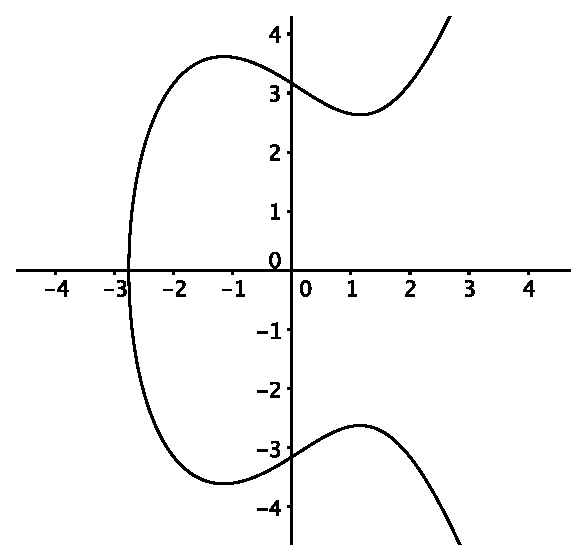
\includegraphics[]{images/curve.eps}
\caption{The elliptic curve $Y^2 = X^3 - 4X + 10$.}
\label{fig:curve}
\end{figure}

\clearpage
\subsubsection{Addition Over Elliptic Curves}

What makes these curves special is that there is a natural way of ``adding''
two points on this curve which always results in a third point which is also on
the curve! This property, combined with a special point $\mathcal{O}$, form an abelian
group in the solution set of an elliptic curve. The point $\mathcal{O}$ serves
as an indentity element, which is said to lie ``at infinity'', or at every
vertical. The elliptic curve addition algorithm is as follows.

\begin{algorithm}
\begin{algorithmic}[]
    \Ensure $E \leftarrow Y^2 = X^3 + AX + B \textbf{ and } 4A^3 + 27B^2 \neq 0$
    \Require $P_1, P_2 \leftarrow \text{some points on E}$
    \If {$P_1 \textbf{ or } P_2 = \mathcal{O}$}
        \If {$P_1 = \mathcal{O}$}
            \Return $P_1 + P_2 = P_2$
        \Else
            \Return $P_1 + P_2 = P_1$
        \EndIf
    \Else
        \State $P_1 = (x_1, y_1)$
        \State $P_2 = (x_2, y_2)$
        \If {$x_1 = x_2 \textbf{ and } y_1 = -y_2$}
            \Return $P_1 + P_2 = \mathcal{O}$
        \Else
            \State $\lambda \leftarrow \left\{
                \begin{array}{l l}
                    \dfrac{y_2 - y_1}{x_2 - x_1} & \quad \text{if $P_1 \neq P_2$}\\\\
                    \dfrac{3x_1^2 + A}{2y_1} & \quad \text{if $P_1 = P_2$}\\
                \end{array}
                \right.$
            \State $x_3 \leftarrow \lambda^2 - x_1 - x_2$
            \State $y_3 \leftarrow \lambda(x_1 - x_3) - y_1$
            \State $P_3 = (x_3, y_3)$
            \Return $P_1 + P_2 = P_3$
        \EndIf
    \EndIf
\end{algorithmic}
\caption{Elliptic curve addition algorithm}
\end{algorithm}

For example, consider the elliptic curve $E: Y^2 = X^3 + 8X + 4$, and the
points $P_1 = (4, 10), P_2 = (5, 13)$, both of which are on the curve.

If we add the two points together using the algorithm above,
\begin{align*}
    \lambda = \frac{13 - 10}{5 - 4} &= 3\\
    x_3 = 3^2 - 4 - 5 &= 0\\
    y_3 = 3(4) - 10 &= 2\\
    P_1 + P_2 &= (0, 2)
\end{align*}
We obtain the point $P_3 = (0, 2)$, which is also a solution to $E$!
\begin{align*}
    2^2 = 0^3 + 8(0) + 4
\end{align*}

The elliptic curve addition can also be demonstrated geometrically.

\begin{figure}[h]
\centering
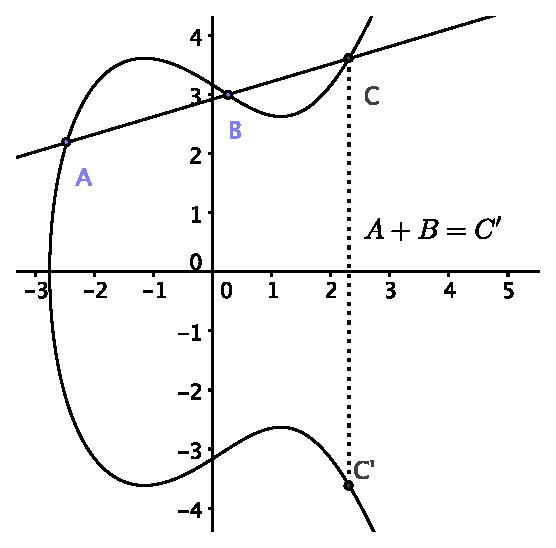
\includegraphics[scale=0.8]{images/add-desc.eps}
\caption{The addition of the points $A + B = C$ on the elliptic
curve $Y^2 = X^3 - 4X + 10$.}
\label{fig:add}
\end{figure}

Suppose we wish to add points $A$ and $B$ on the elliptic curve $E$. We start
by drawing a line between these points, $L$. Due to the structure of the
curve, $L$ also intersects $E$ at another point $C$. This point $C$ is reflected
over the $x$-axis to obtain the point $C'$, which is the elliptic sum of
$A$ and $B$. See Figure \ref{fig:add} for an illustration of this process.

\subsubsection{Elliptic Curves Over Finite Fields}

To allow for us to work with elliptic curves in a cryptographic
context we need to extend our definition of elliptic curves to
include elliptic curves over finite fields. This will allow
us to define the mathematically difficult problem which defines
the security of the ElGamel cipher.

Simply, we defined elliptic curves whose points have coordinates
in the finite field (``over'' the finite field) $\mathds{F}_p$, with
the equation
\begin{align*}
    E:Y^2 = X^3 + AX + B \text{ with } A, B \in \mathds{F}_p \text{ satisfiying }
    4A^3 + 27B^2 \neq 0
\end{align*}
where $p$ is some prime number larger than 3. The points on $E$ with
coordinates in $\mathds{F}_p$ are denoted by
\begin{align*}
    E(\mathds{F}_p) = \{ (x, y): x, y \in \mathds{F}_p \text{ and } y^2 = x^3 + Ax + B \} \cup \{ \mathcal{O} \}
\end{align*}

The same addition rule we previously defined works here as well, however,
because all operations are now in the field $\mathds{F}_p$, the addition
of two points will always yield another point inside $\mathds{F}_p$. This
cyclic property of the group is what this cipher exploits to ensure its
security.

For example, consider the addition of the points $P_1 = (0, 2), P_2 = (4, 10)$ on
the elliptic curve $E:Y^2 = X^3 + 8X + 4$ over the finite field $\mathds{F}_{11}$.
\begin{align*}
    \lambda = \frac{10 - 2}{4 - 0} &\equiv 2 \pmod{11}\\
    x_3 = 2^2 - 0 - 4 &\equiv 0 \pmod{11}\\
    y_3 = 2(0) - 2 &\equiv 9 \pmod{11}\\
    P_1 + P_2 &= (0, 9)
\end{align*}
Although it may not seem obvious,
\begin{align*}
    9^2 &\equiv 0^3 + 8(0) + 4 \pmod{11}\\
    81 &\equiv 4 \pmod{11}
\end{align*}
The point $(0, 9)$ is indeed a solution to $E$ in the field $\mathds{F}_{11}$.

\subsubsection{Elliptic Curve Discrete Logarithm Problem}

As we mentioned earlier, the elliptic curve discrete logarithm problem (ECDLP),
is the underlying hard problem upon which ElGamel is based.

The ECDLP is the problem of finding and integer $n$ such that
$Q = nP$, where $P, Q \in E(\mathds{F}_p)$ and the multiplication of $n$ and
$P$ is defined as:
\begin{align*}
    \underbrace{P + P + P + \cdots + P}_{\text{$n$ additions over $E$}} = nP = Q
\end{align*}

Althougth this may seem simple, remember that the addition occuring over the
curve $E$ more complex than normal addition, and that it is being done in the
field $\mathds{F}_p$.

A key point to notice here is that if there exists one $n$ then there must,
through the cyclic nature of the addition rule, be an infinite number of
$n$ which also solve $Q = nP$. As we shall soon see, this can be exploited to
find $n$.

%For example, given the points $P = (0, 2), Q = (0, 9)$ on the elliptic curve
%$Y^2 = X^3 + 8X + 4$ in the field $\mathds{F}_{11}$, it turns out that
%\begin{align*}
%    19P = 29P = Q\\
%\end{align*}
%In fact, any $n$ of the form $9 + 10k$, where $k \in \mathds{Z}^+$, will
%give us a multiple
% 10 is the order of E(F_P)!!;

\subsection{Elliptic ElGamel}

Now that we have an understanding of the mathematics behind elliptic curves and
the ECDLP, we can describe the ElGamel cipher in its entirety.

ElGamel works as follows. A large prime $p$, an elliptic curve $E$ over
$\mathds{F}_p$ and a point $P \in E(\mathds{F}_p)$ are chosen by a trusted
party or agreed upon by Alice and Bob and published to the public. Alice then
chooses a private key, $n_A$, and computes $Q_A = n_AP$ in $E(\mathds{F}_p)$.
She then published $Q_A$ as her public key. If Bob wants to send a message to
Alice, he chooses a plaintext $M \in E(\mathds{F}_p)$ and a temporary key $k$.
He then computes $C_1 = kP$ and $C_2 = M + kQ_A$ in $E(\mathds{F}_p)$ and sends
$(C_1, C_2)$ to Alice. Alice then computes $C_2 - n_AC_1$ in $E(\mathds{F}_p)$
to obtain $M$, given that:
\begin{align*}
    C_2 - n_AC_1 = (M + kQ_A) - n_A(kP) = M + k(n_AP) - n_A(kP) = M
\end{align*}

To illustrate this cipher in action let us assume there is a public point
$P = (6, 730)$ on the elliptic curve $E:Y^2 = X^3 + 14X + 19$ in the finite
field $\mathds{F}_{3623}$. Alice pickes a secret key $K_{pri} = 12$ and
publishes her private key
\begin{align*}
    K_{pub} = 12P = (1669, 1991)
\end{align*}
Bob wants to send Alice the message $M = (2149, 196)$, so he picks a temporary
key $k = 4$ and computes
\begin{align*}
    C_1 &= kP = 4P = (2277, 502)\\
    C_2 &= M + k(K_{pub}) = (2149, 196) + (1175, 1246) = (600, 2449)
\end{align*}
Which he then sends to Alice. Upon receiving $C_1$ and $C_2$, Alice computes
\begin{align*}
    M = C_2 - K_{pri}C_1 = (2277, 502) - (1175, 1246) = (2149, 196)
\end{align*}
Which was indeed what Bob sent her. Notice that all Eve saw during this entire
transaction were the points $C_1$ and $C_2$, both of which require knowing
either the temporary key, $k$, or the private key, $K_{pri}$ before
they can be deciphered, which in turn, requires solving ECDLP.

\subsection{The Birthday Paradox and the Collision Theorem}

Now that we have described the algorithm, let us take a quick tangent into
the realm of probability theory which we shall use, in conjunction to our
knowledge that and infinite number of solutions exist to the ECDLP, to
cryptanalyse our cipher.

\subsubsection{The Birthday Paradox}

Given a group of 40 people, consider the following questions:

\begin{enumerate}
\item What is the probability that someone has the same birthday as you?
\item What is the probability that at least two people have the same birthday?
\end{enumerate}

Contrary to popular belief, the answers to these questions vary greatly. In
the first case, the probability can be calculated by determining the
probability that none of these people share your birthday, and subtracting
this by 1.
\begin{align*}
    \ptm{someone has}{your birthday} & = 1 - \ptm{no one has}{your birthday}\\
    & = 1 - \prod_{i = 1}^{40}\ptm{the $i^{\text{it}}$ person does not}{have your birthday}\\
    & = 1 - \left(\frac{364}{365}\right)^{40}\\
    & \approx 10.4 \%
\end{align*}
Note that the probability of this occuring is not $\frac{40}{365}$ as this
method double counts the occurence of more than one person who shares your
birthday.

Now consider the second case, where we calculate the probability that two
people of this group of 40 have the same birthday. In this case we need
to calculate the probability that each $i^{th}$ person has a different
birthday than the previous $i - 1$ people. Therefore, we obtain:
\begin{align*}
    \ptm{two people have}{the same birthday} & = 1 - \ptm{all 40 people have}{different birthdays}\\
    & = 1 - \prod_{i = 1}^{40}\ptm{the $i^{\text{th}}$ person does not have the same birthday}
    {as any of the previous $i - 1$ people}\\
    & = 1 - \prod_{i = 1}^{40}\frac{365 - (i - 1)}{365}\\
    & \approx 89.1 \%
\end{align*}
It is worth noting how we have arrived at the formula for the probability of the
$i^{\text{th}}$ person not having the same birthday as any of the previous
$i - 1$ people. If the $i^{\text{th}}$ person is to have a birthday which is
different from any of the previous $i - 1$ people, he only has $365 - (i - 1)$
choices of dates which have not been repeated. Therefore, the probability
that he has a birthday on one of those dates is simply $\frac{365 - (i - 1)}
{365}$.

The surprising thing is that most people assume 1 and 2 have relatively similar
probabilities, when in fact the former event has a probability of approximately
10\% whereas the latter event has a probability of approximately 90\%. The idea
that finding two identical objects in a set is easier than finding a match for
one is the basis of cryptographic collisions. Broadly, a cryptographic collision
can be defined as the event which occurs when two objects in a large set of
(often distinct) objects are identical.

\subsubsection{The Collision Theorem}

The Collision Theorem states that given a total of $N$ possible objects,
and two distinct subsets of those objects $A$ where $|A| = n$, and $B$ where
$|B| = N - n$, the probability of choosing at least one object from $A$ after
$m$ random choices is
\begin{align}
    \Pr\left(\text{at least object from $A$}\right) = 1 - \left(1 - \frac{n}{N}\right)^m
\end{align}
And that the following is a lower bound for $(2)$
\begin{align}
    \Pr\left(\text{at least object from $A$}\right) \geq 1 - e^{-mn/N}
\end{align}
Furthermore, it turns out that when $n$ and $m$ are not too much larger than
$\sqrt{N}$, $(3)$ is almost an equality.

For example, suppose that we are given two random lists of names which are $1000$
names long from a phone book with $1,000,000$ names. What is the probability
that a name from our two lists is identical? The Collision Theorem says
\begin{align*}
    \Pr\left(\text{a match}\right) = 1 - \left(1 - \frac{1000}{10^6}\right)^{1000} \approx 63.2 \%
\end{align*}
If we take a look at the lower bound
\begin{align*}
    \Pr\left(\text{a match}\right) \geq 1 - e^{-1000(1000)/10^6} \approx 63.2 \%
\end{align*}
We see that they are quite similar.

Now suppose that instead of a list of $1000$ names, we were given a list of $4000$
names. Note that $4000 = 4(1000) = 4\sqrt{10^6}$ is a small multiple of $\sqrt{N}$. Now, our
results are quite different
\begin{align*}
    \Pr\left(\text{a match}\right) = 1 - \left(1 - \frac{4000}{10^6}\right)^{4000} \approx 99.9 \%
\end{align*}
And our lower bound is equally high
\begin{align*}
    \Pr\left(\text{a match}\right) \geq 1 - e^{-4000(4000)/10^6} \approx 99.9 \%
\end{align*}

The proof of this theorem is beyond the scope of this report, however, if you
are curious you can find it in \cite[p.~227]{silverman}.

\subsection{Cryptanalysis of the ElGamel Cipher}

We know that if we solve the underlying hard problem of the ElGamel cipher
namely, ECDLP, then we can quite easily break the entire cipher, as ElGamels
public key $Q_A = n_AP$ relies on the intractability of the ECDLP to maintain
the secrecy of $n_A$. The naive solution would be the check every value of
$n$ less than than the order of the finite field $\mathds{F}_p$, however, this
will quickly become infeasible as large $p$ are chosen, take a total time of
$O(p)$.

Consider the following solution to the ECDLP, using the Shank's Baby Step
Giant Step algorithm adapted for the ECDLP. We shall create two lists of
multiples of the points:
\begin{description}
    \item[\quad List 1.] \quad $j_1P, j_2P, j_3P, \ldots, j_rP$
    \item[\quad List 2.] \quad $k_1P + Q, k_2P + Q, k_3P + Q, \ldots, k_rP + Q$
\end{description}
Where $j_1, \ldots, j_r$ and $k_1, \ldots, k_r$ are between 1 and $p$.
As soon as we find a collision between these two lists, it becomes trivially
easy to compute $nP = Q$, as:
\begin{align*}
    j_uP &= k_vP + Q\\
    (j_u - k_v)P &= Q
\end{align*}
Therefore $n = (j_u - k_v)$.

We also know from the Collison Theorem, that the size of List 1 and List 2 need
only be a small multiple of the size of $\sqrt{p}$, after which the probability
of a match is very high.

It is clear that this method is considerably faster than exhaustive search as
each list requires only $2\sqrt{p}$ operations to create, given each step is an
elliptic multiplication. Comparing the lists should also only take a maximum of
$2\sqrt{p}$ operations. Therefore, this algorithm should run in approximately
$O(\sqrt{p})$ time.

To illustrate the effectiveness of this algorithm, consider solving ECDLP
for the points $P = (1395, 8021)$ and $Q = (10866, 8078)$ on the elliptic curve
$E:Y^2 = X^3 + 43X + 93$ in the field $\mathds{F}_{22307}$. On my machine,
the Shank's ECDLP adaptation requires between 17 and 19 milliseconds to run,
where as exhaustive search requires approximately 303 milliseconds. This supports
our claim that Shank's ECDLP adaptation runs in time $O(\sqrt{p})$ as
$\sqrt{303} \approx 17.5$.

\subsection{Advantages and Disadvantages of the ElGamel Cipher}

Clearly, the overwhelming advantage of ElGamel is that it will always be secure,
so long as there is no efficient algorithm to solve the ECDLP, irrespective
of any other factor\fnt{This is not entirely true, as in certain cases, such as
when an elliptic curve is anomalous, it is possible to solve ECDLP in $O(\ln p)$.
For a much deeper investigation of such rare cases, see \cite{musson}.}. Informally,
this means that we can choose certain primes, $p$, such that the running time
for the most efficient algorithm to solve ECDLP, $O(\sqrt{p})$ is too high to
ever be computed in a feasible amount of time\fnt{For example, the expected age of
the universe.}.

Despite this theoretic security, ElGamel remains solemn used in practise for
one key reason. There is so obvious way to store a message using a point!
Therefore, ElGamel is often used in conjunction with other symmetric key ciphers
(primarily block ciphers) to securely exchange keys with multiple parties.

Furthermore, ElGamel requires very large keys in comparison to symmetric
ciphers. For example, to achieve a security of 128 bits, one requires an elliptic
curve over a finite field $\mathds{F}_p$ where $p \approx 2^{256}$, as this
means an attacker would need to compute $\sqrt{2^{256}} = 2^{128}$ operations.
In contrast, block ciphers only require keys of size $2^{128}$.

However, in comparison to other public-key ciphers, ElGamel performs remarkably
well. To achieve 128 bit security using conventional public-key ciphers\fnt{
See \cite{nsa} for more information regarding these statistics.}
such as RSA, one requires keys of size $2^{3072}$! This means that ElGamel
is 10 times more memory efficient! Furthermore, as the power of computers,
increases, ElGamel scales much better as a higher security level is required.
If suppose, in 10 years, a security of 256 bits is required, ElGamel would
only require $p \approx 2^{512}$, whereas RSA would require keys of size
$2^{15360}$!

\section*{Conclusions and Further Exploration}
\addcontentsline{toc}{section}{Conclusions and Further Exploration}

In this paper, we have analyzed a variety of cryptographic algorithms which are
essential to modern cryptography: substitution ciphers, block ciphers, and
public-key ciphers. We have evaluated the utility of each cipher not only with
respect to their security, but also to their practicality, speed and
memory efficiency. Furthermore, we have learnt to employ many advanced
cryptanalytic techniques, from simple frequency analysis attacks to advanced
collision attacks.

Moving forward, there are several other more advanced branches of cryptography
which have not been addressed in this paper, despite their prevalence in modern
cryptography. These topics include cryptographic hashing, random number
generation, quantum cryptography, digital authentication, hyper elliptic curve
cryptography and digital signatures. These topics were not included in this
paper as their complexity is beyond the abilities of the author. However,
I encourage the reader to see \cite{silverman,schneier} for more information. I
hope you have enjoyed learning about cryptography as much as I have.

\clearpage
\bibliographystyle{plain}
\bibliography{doc.bib}

\clearpage
\section*{Appendix}
\addcontentsline{toc}{section}{Appendix}

All of the following code is also available online at the following locations:
\begin{description}
    \item[\quad Caesar Cipher] \url{http://bit.ly/JYyL3L}
    \item[\quad GHOST Cipher] \url{http://bit.ly/J5lGAF}
    \item[\quad ElGamel Cipher] \url{http://bit.ly/IlyrYL}
\end{description}
The Caesar cipher and the GHOST cipher need to be compiled using the
\texttt{GCC} source compiler.

The ElGamel cipher needs to be run using \texttt{node.js}. To install
\texttt{node.js}, visit \url{http://nodejs.org/}.

\subsection*{Caesar Cipher Source Code}
\addcontentsline{toc}{subsection}{Caesar Cipher Source Code}
\subsubsection*{caesar.c}
\inputminted[fontsize=\scriptsize]{c}{code/caesar.c}

\subsection*{GHOST Cipher Source Code}
\addcontentsline{toc}{subsection}{GHOST Cipher Source Code}
\subsubsection*{ghost.h}
\inputminted[fontsize=\scriptsize]{c}{code/ghost.h}
\subsubsection*{ghost.c}
\inputminted[fontsize=\scriptsize]{c}{code/ghost.c}
\subsubsection*{main.c}
\inputminted[fontsize=\scriptsize]{c}{code/main.c}

\subsection*{ElGamel Cipher Source Code}
\addcontentsline{toc}{subsection}{ElGamel Cipher Source Code}
\subsubsection*{point.js}
\inputminted[fontsize=\scriptsize]{javascript}{code/point.js}
\subsubsection*{curve.js}
\inputminted[fontsize=\scriptsize]{javascript}{code/curve.js}
\subsubsection*{elgamel.js}
\inputminted[fontsize=\scriptsize]{javascript}{code/elgamel.js}
\subsubsection*{main.js}
\inputminted[fontsize=\scriptsize]{javascript}{code/main.js}
\end{document}
